%%%%%%%%%%%%%%%%%%%%%%%%%%%%%%%%%%%%%%%%%%%%%%%%%%%%%
%%% Task 2 %%%%%%%%%%%%%%%%%%%%%%%%%%%%%%%%%%%%%%%%%%
%%%%%%%%%%%%%%%%%%%%%%%%%%%%%%%%%%%%%%%%%%%%%%%%%%%%%
\task{DC machine}

%%%%%%%%%%%%%%%%%%%%%%%%%%%%%%%%%%%%%%%%%%%%%%
\taskGerman{DC Maschine}

\subtask{What are the three main connection types for DC machines? Draw the 
equivalent circuit diagrams and add the respective current and voltage equations in the steady state.}{3}

\subtaskGerman{Welche drei wesentlichen Schaltungsarten gibt es für Gleichstrommaschinen? Zeichnen Sie die 
Ersatzschaltbilder mit den jeweiligen Strom- und Spannungsgleichungen im stationären Zustand.}

\begin{solutionblock}
The three types are:

Series DC machine:
$$ U = U_\mathrm{a} + U_\mathrm{f} = (R_\mathrm{a} + R_\mathrm{f}) I + \omega L'_\mathrm{f} I, \qquad I = I_\mathrm{a} = I_\mathrm{f}.$$ 
\begin{center}
    \includegraphics[width=0.5\textwidth]{../../lecture/fig/lec03/Series_DC_machine.pdf}
\end{center}

Shunt DC machine:
$$ U = U_\mathrm{a} = U_\mathrm{f}, \quad I = I_\mathrm{a} + I_\mathrm{f}, \quad I_\mathrm{f} = \frac{U_\mathrm{f}}{R_\mathrm{f}}, \quad I_\mathrm{a} = \frac{1-L'_\mathrm{f}/R_\mathrm{f}\omega}{R_\mathrm{a}}U$$
\begin{center}
    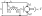
\includegraphics[width=0.5\textwidth]{../../lecture/fig/lec03/Shunt_DC_machine.pdf}
\end{center}

Separately-excited DC machine:
$$ U_\mathrm{a} = R_\mathrm{a} I_\mathrm{a} + \omega L'_\mathrm{f} I_\mathrm{f}, \quad U_\mathrm{f} = R_\mathrm{f} I_\mathrm{f}$$
\begin{center}
    
\includegraphics[width=0.5\textwidth]{../../lecture/fig/lec03/Separately_excited_DC_machine.pdf}
\end{center}
\end{solutionblock}

\subtask{Now consider a DC machine with the parameters given in \autoref{tab:characteristicsDC_task2}. To which of the above connection type can the parameter set belong?}{1}
\subtaskGerman{Betrachten Sie nun eine Gleichstrommaschine mit den Parametern aus \autoref{tab:characteristicsDC_task2}. Zu welchen der obigen Verschaltungsarten kann dieser Parametersatz gehören?}
\begin{table}[htb]
    \caption{Characteristics of the given DC machine.}
    \centering
    \begin{tabular}{lll}\toprule
    Symbol  & Description       & Values \\
    \midrule
    $U_{\mathrm{a,n}}$    & Nominal armature voltage           & $\SI{230}{\volt}$ \\
    $I_{\mathrm{a,n}}$    & Nominal armature current           & $\SI{20}{\ampere}$ \\
    $U_{\mathrm{f,n}}$    & Nominal field voltage           & $\SI{230}{\volt}$ \\
    $I_{\mathrm{f,n}}$    & Nominal field current           & $\SI{1.1}{\ampere}$ \\
    $R_{\mathrm{a}}$    & Armature resistance           & $\SI{1.2}{\ohm}$ \\
    $R_{\mathrm{f}}$    & Field resistance           & $\SI{42.0}{\ohm}$ \\
    $P_{\mathrm{n}}$    & Nominal power             & $\SI{4.1}{\kilo\watt}$ \\
    $n_{\mathrm{n}}$    & Nominal speed             & $\SI{1500}{\per\minute}$\\ 
    \bottomrule
    \end{tabular}
    \label{tab:characteristicsDC_task2}
\end{table}

\begin{solutionblock}
    Since the field and armature voltage are equal while their currents are different, the machine could be a shunt DC machine. However, a seperately-excited DC machine could also be possible if two different power supplies are used for the field and armature. 
\end{solutionblock}

\subtask{Calculate the nominal torque $T_\mathrm{n}$.}{2}
\subtaskGerman{Berechnen Sie das Nenndrehmoment $T_\mathrm{n}$.}

\begin{solutionblock}
    The nominal mechanical power is given by
    $$ P_{\mathrm{n}} = T_{\mathrm{n}} \omega_{\mathrm{r,n}}=T_{\mathrm{n}} 2\pi n_{\mathrm{n}} \SI{\frac{1}{60}}{\minute\per\second}.$$
    Hence, we can calculate the nominal torque as
    $$ T_{\mathrm{n}} = \frac{P_{\mathrm{n}}}{n_{\mathrm{n}}} \cdot\frac{ 60}{2\pi } \si{\second\per\minute}= \SI{26.1}{\newton\meter}.$$
\end{solutionblock}

\subtask{Determine the nominal efficiency $\eta_\mathrm{n}$ of the entire machine.}{2}
\subtaskGerman{Bestimmen Sie den Nennwirkungsgrad $\eta_\mathrm{n}$ der gesamten Maschine.}

\begin{solutionblock}
    The nominal electrical power is
    $$ P_{\mathrm{el,n}} = U_{\mathrm{a,n}} I_{\mathrm{a,n}} + U_{\mathrm{f,n}} I_{\mathrm{f,n}} = \SI{230}{\volt} \cdot \SI{20}{\ampere} + \SI{230}{\volt} \cdot \SI{1.1}{\ampere} = \SI{4853}{\watt}.$$
    The efficiency is then
    $$ \eta_\mathrm{n} = \frac{P_{\mathrm{n}}}{P_{\mathrm{el,n}}} = \frac{\SI{4100}{\watt}}{\SI{4853}{\watt}} = 0.85 = \SI{85}{\percent}. $$
\end{solutionblock}

\subtask{Calculate the armature starting current $I_\mathrm{a,0}$  and the resulting starting torque $T_0$.}{2}
\subtaskGerman{Berechnen Sie den Ankeranlaufstrom $I_\mathrm{a,0}$ und das resultierende Anlaufdrehmoment $T_0$.}

\begin{solutionblock}
    The armature starting current is given by
    $$ I_{\mathrm{a,0}} = \frac{U_{\mathrm{a,n}}}{R_{\mathrm{a}}} = \frac{\SI{230}{\volt} }{\SI{1.2}{\ohm}}  = \SI{191.67}{\ampere}.$$
    For the torque we first calculate the effective field excitation 
    $$ T_\mathrm{n} = \psi'_\mathrm{f} I_\mathrm{a,n} \quad \Leftrightarrow \quad \psi'_\mathrm{f} = \frac{T_\mathrm{n}}{I_\mathrm{a,n}} = \frac{\SI{26.1}{\newton\meter}}{\SI{20}{\ampere}} = \SI{1.305}{\volt\second}$$
    and then the starting torque
    $$ T_0 = \psi'_\mathrm{f} I_{\mathrm{a,0}} = \SI{1.305}{\volt\second} \cdot \SI{191.67}{\ampere} = \SI{250.13}{\newton\meter}.$$
\end{solutionblock}

\subtask{Discuss potential operation issues of the found starting torque and current values compared to the machine's nominal operation. Propose  potential remedies to address these issues.}{2}
\subtaskGerman{Diskutieren Sie mögliche Betriebsprobleme der gefundenen Anlaufdrehmoment- und Stromwerte im Vergleich zum Nennbetriebspunkt der Maschine. Schlagen Sie mögliche Lösungen vor, um diese Probleme zu beheben.}

\begin{solutionblock}
    The starting current is significantly higher than the nominal current, which can lead to thermal issues in the machine. The starting torque is also higher than the nominal torque, which can lead to mechanical issues. To address these issues, potential remedies could be:
    \begin{itemize}
        \item Vary the armature voltage by an adaptive power supply. 
        \item Vary the field excitation by an adaptive power supply (if separately-excited type).
        \item Introduce dropping resistors in the armature circuit during starting.
    \end{itemize}
    If these remedies are necessary highly depends on the specific application of the machine and in particular how fast the machine is accelerated as this will reduce the armature current due to the induced voltage. 
\end{solutionblock}